\documentclass[12pt]{article}
\usepackage{graphicx}
\usepackage{amsmath}
\usepackage{amssymb}
\usepackage{pifont}
\usepackage[margin=0.65in]{geometry}
\usepackage{enumerate}
\usepackage{caption}
\usepackage{float}
\usepackage{graphicx}
\usepackage{subfig}\usepackage{graphicx}
\usepackage{subfig}
\usepackage{program}

\def\arraystretch{1.5}
\captionsetup{aboveskip=8pt}
\newcommand{\cmark}{\ding{51}}%
\newcommand{\xmark}{\ding{55}}%
\setlength{\parskip}{1em}

\begin{document}
\title{MISDC Writeup}
\author{Will Pazner}
\maketitle

\section{Background}
We are currently using a modified MISDC algorithm in the low Mach number 
combustion code to solve an system of advection-diffusion-reaction 
equations. The code is stable, and second-order accurate. We are investigating 
potential modifications to the code with the end-goal of increasing the order 
of accuracy.

The equations of interest can be written in the form
\begin{equation}
    \frac{\partial \phi}{\partial t}(t) = A(\phi) + D(\phi) + R(\phi) = F(\phi)
\end{equation}
where $A$, $D$, and $R$ represent the advection, diffusion, and reaction 
processes, respectively. Because of the different time-scales involved, the 
goal is to use a multi-implicit method, where advection is treated explicitly, 
and diffusion and reaction are treated implicitly.
\subsection{Note on current implementation}
Currently, we solve a system of ``weakly coupled'' equations at each time step. 
They are given by
\begin{flalign}
    \label{adv-corr}
    \phi_A^{(k+1)}(t) &= \phi^n + \int_{t^n}^t \left( A(\phi_A^{(k+1)}) 
                                              - A(\phi^{(k)})\right) d\tau
                               + \int_{t^n}^t F(\phi^{(k)}) d\tau &&\\
    \label{dif-corr}
    \phi_{AD}^{(k+1)}(t) &= \phi^n + \int_{t^n}^t
                                    \left( A(\phi_A^{(k+1)}) - A(\phi^{(k)})
                                         + D(\phi_{AD}^{(k+1)} - D(\phi^{(k)}))
                                    \right) d\tau
                                  + \int_{t^n}^t F(\phi^{(k)}) d\tau &&\\
    \nonumber
    \phi^{(k+1)}(t) &= \phi^n + \int_{t^n}^t
                                 \Big( A(\phi_A^{(k+1)})    - A(\phi^{(k)}
                                     + D(\phi_{AD}^{(k+1)}) - D(\phi^{(k)})\\
    \label{corr} & \hspace{2.5 in}     + R(\phi^{(k+1)})      - R(\phi^{(k)})
                                 \Big) d\tau
                              + \int_{t^n}^t F(\phi^{(k)})  d\tau
\end{flalign}
The order of accuracy of the method is limited by the accuracy of the quadrature 
rule used to compute $\int_{t^n}^t F(\phi^{(k)})  d\tau$. In the current 
implementation a two-point trapezoidal rule is used for the advection and 
diffusion, and the integral of the reaction term (represented as $I_R$) is 
computed analytically using equation (\ref{corr}). The integrals immediately 
following $y^n$ in equations (\ref{adv-corr}~-~\ref{corr}) can be computed using 
a simple first-order quadrature.

The advection correction equation (\ref{adv-corr}) is solved using an explicit 
Forward Euler step, and the diffusion correction equation (\ref{dif-corr}) is 
solved using an implicit Backward Euler step.

We note that in solving the final correction equation, we differ 
from the ``classic'' MISDC algorithm. Instead of solving the integral equation 
(\ref{corr}) using a simple Backward Euler step, we instead differentiate 
equation (\ref{corr}) to obtain an ordinary differential equation. The resulting 
ODE is
\begin{equation}
\phi^{(k+1)}_t = D(\phi_{AD}^{(k+1)}) - D(\phi^{(k)}) + R(\phi^{(k+1)})
                      - R(\phi^{(k)}) + F(\phi^{(k)}).
\end{equation}
The main question of interest is how to represent the term $F(\phi^{(k)})$. 
In the LMC code, $F$ is represented as
\begin{equation}
    F(\phi^{(k)}) \approx \frac{1}{2}\left(
        A(\phi^n) + D(\phi^n) + A(\phi^{(k),n+1})+D(\phi^{(k),n+1})
        \right) + R(\phi^{(k)}).
\end{equation}
In other words, the advection and diffusion terms are treated as piecewise 
constants, whose value is the average at the current and next timesteps. The 
reaction term is considered exact, and cancels with the corresponding reaction 
term from the first integral. We are left with the ODE
\begin{equation}
\phi^{(k+1)}_t = R(\phi^{(k+1)},t) + D(\phi_{AD}^{(k+1),n+1})
                 + \frac{1}{2}\left(A(\phi^n) + D(\phi^n) + 
                    A(\phi^{(k+1),n+1})-D(\phi^{(k+1),n+1})\right).
\end{equation}
This ODE is then solved using VODE in order to obtain the final solution at the 
next timestep.
\subsection{Piecewise linear forcing}\label{lmc-linear-forcing}
In order attain higher than second-order accuracy, the quadrature rule used in 
computing $\int_{t^n}^t F(\phi^{(k)})  d\tau$ must be higher order. In other 
words, $F(\phi^{(k)})$ must be represted by a higher degree polynomial. As a 
first step towards this, instead of represting $F(\phi^{(k)})$ as a piecewise 
constant given by the average value, we consider $F(\phi^{(k)})$ to be the 
piecewise linear function give by
\begin{equation}
    F(\phi^{(k)}) \approx \left(1-\frac{t}{\Delta t}\right)\left(
        A(\phi^n) + D(\phi^n)\right) + \frac{t}{\Delta t} \left(
        A(\phi^{(k),n+1})+D(\phi^{(k),n+1})
        \right) + R(\phi^{(k)}).
\end{equation}
When this change is attempted in the code, the resulting method is unstable. 
For fixed spatial resolution, choosing a sufficiently small $\Delta t$ results 
in stability, but, for example, refining $\Delta x$ by a factor of 2 requires 
$\Delta t$ to be refined by more than a factor of 4.

Additionally, we notice that the method diverges not only as we advance in time, 
but also for a single time step, when the number of MISDC iterations is taken 
to be large. This suggests to us that the MISDC iterative scheme is failing to 
converge to its fixed point.

It it also worth noting that using a piecewise linear function to represent the 
advection term, and a piecewise constant term to represent the diffusion term 
results in a stable method. This suggests that it is the reaction and diffusion 
processes that result in the instability, and that the advection is largely 
irrelevent.
\section{Simple Linear ODE}\label{sec:ode}
In order to further study the MISDC algorithm when applied to an advection-%
diffusion-reaction equation, we consider the simple linear ODE
\begin{equation}
    \label{lin}
    y' = ay + dy + ry, \qquad y(0) = 1
\end{equation}
where $a$, $d$ and $y$ represent advection, diffusion, and reaction terms 
respectively. The exact solution is given by $e^{(a+d+r)t}$. The value of $d$ 
is chosen to be negative because of the negative eigenvalues of the Laplacian 
operator. $r$ is chosen to be positive to ``balance'' the effect of the 
diffusion.

We want to solve this ODE using an MISDC-like iterative scheme. 
As in the LMC code, we solve for advection explicitly (Forward Euler) and 
for diffusion implicitly (Backward Euler). Because of the structure of the 
scheme, we never have to calculate the intermediate advection solution. Then, we 
are left with a correction equation for reaction of the form
\begin{equation}
\label{lin-corr}
\begin{split}
    y^{(k+1)}(t) = y^n + \int_{t^n}^t \Big(
        A(y^{(k+1)}_A) - A(y^{(k)})
      + D(y^{(k+1)}_{AD}) - D(y^{(k)}) \\
      + R(y^{(k+1)}) - R(y^{(k)})
      \Big) d\tau
      + \int_{t^n}^t F(y^{(k)}) d\tau.
\end{split}
\end{equation}
In the two-node case, $A(y^{(k+1)}_A)$ and $A(y^{(k)})$ exactly cancel.
This equation can be solved in a number of ways:
\begin{enumerate}[I.]
    \item  The ``classical MISDC'' method approximates the first integral using 
           a first order quadrature rule, and the second integral using a 
           higher-order quadrature rule, solving for $y^{(k+1)}$ using a 
           Backward Euler step. \label{classic-misdc}
    \item  The method used by LMC, which is similar to a ``deferred correction'' 
           scheme rather than ``spectral deferred correction,'' differentiates 
           equation (\ref{lin-corr}) to obtain a differential equation. This 
           equation can then be solved using a variety of methods (\textit{e.g.} 
           RK-4, VODE ODE solver, using an analytical solution derived by hand, 
           etc.). If $\int_{t^n}^t F(y^{(k)}) d\tau$ is approximated using a 
           higher-order quadrature rule, this corresponds to a higher-degree 
           polynomial for the forcing term. \label{misdc-ode}
\end{enumerate}

\subsection{Polynomial representation of forcing term}
As in section \ref{lmc-linear-forcing}, in order to increase the order of 
accuracy, we need to increase the order of the underlying quadrature rule 
(and therefore increase the number of substeps or nodes at which the solution 
is calculated). This correspondings to increasing the degree of the underlying 
polynomial representation of the solution.

The simplest representation of the forcing term is a piecewise constant, 
given by the average at the current and next timesteps:
\begin{gather}
    A_0(y^{(k)}) := \frac{1}{2} \left( A(\phi^{(k),n}
                                        + A(\phi^{(k),n+1} \right) \\
    D_0(y^{(k)}) := \frac{1}{2} \left( D(\phi^{(k),n}
                                        + D(\phi^{(k),n+1} \right).
\end{gather}
(Here, the subscript indicates the degree of polynomial used to represent the 
forcing term). This corresponds to the representation currently used in the LMC 
code.

We can also choose a piecewise linear representation:
\begin{gather}
    A_1(y^{(k)}) := \left(1 - \frac{t}{\Delta t}\right) A(\phi^{(k),n}
                            + \frac{t}{\Delta t}        A(\phi^{(k),n+1}\\
    D_1(y^{(k)}) := \left(1 - \frac{t}{\Delta t}\right) D(\phi^{(k),n}
                            + \frac{t}{\Delta t}        D(\phi^{(k),n+1}.
\end{gather}

Finally, we implemented \textit{advection substepping}, where the solution is 
computed at intermediate substeps, and the forcing term is considered to be 
the interpolating polynomial passing through those points. We chose the subteps 
to be given by the Gauss-Lobatto quadrature points:
\begin{align*}
    t_{(0)} &= t^n \\
    t_{(1)} &= t^n + \Delta t \left( \frac{1 - \sqrt{1/5}}{2} \right)\\
    t_{(2)} &= t^n + \Delta t \left( \frac{1 + \sqrt{1/5}}{2} \right)\\
    t_{(3)} &= t^{n+1} = t^n + \Delta t.
\end{align*}
Then, the advection and diffusion forcing terms are considered to be the 
interpolating cubic, with values given at the four points $t_{(j)},$
$j=0,1,2,3$.

In all these cases, the correction ODE is of the form
\begin{equation}
    y' = ry + \mathcal{P}_{AD}(t),
\end{equation}
where $\mathcal{P}_{AD}(t)$ is the polynomial forcing term.

Choosing moderate coefficients for $a$, $d$, and $r$, all of these methods 
result in the expected order of accuracy. Method \ref{misdc-ode} was implemented 
both using a fourth-order Runge-Kutta ODE solver and using the exact solution, 
computed by hand.

\subsection{Nonlinearity}
In order to further test our method, we applied our numerical method to 
the following equations (where $p(t) = cos(t)$, for example)
\begin{gather}
    \label{nonlin}
    y'(t) = ay(t) + dy(t) + ry(t)(y(t) - 1)(y(t) - 1/2)\\
    \label{lincos}
    y'(t) = p'(t) + a(p(t)-y(t)) + d(p(t)-y(t)) + r(p(t) - y(t)) \\
    \label{nonlincos}
    y'(t) = p'(t) + a(p(t)-y(t)) + d(p(t)-y(t)) + ry^2(t)(p(t) - y(t)),
\end{gather}
where equation (\ref{nonlin}) is a nonlinear version of (\ref{lin}), and 
equation (\ref{nonlincos}) is a nonlinear modification of (\ref{lincos}). The 
exact solution to (\ref{lincos}) is given by $p(t)$. In both of these cases, 
the method performed as expected, with the same accuracy and stability 
properties as in the previous section. In contrast to the behavior observed 
in the LMC code, with moderate coefficients chosen for $a$, $d$, and $r$, there 
was no difference in performance or stability between solving the reaction 
correction ODE using a piecewise constant or piecewise linear forcing term.

\subsection{Stability observations}
With ``moderate'' coefficients, piecewise constant, linear and cubic terms all 
result in satisfactory convergence. When the timestep is relatively large, or 
when the coefficients are chosen to be large in magnitude, instability is 
observed. The following table details a small number of numerical experiments. 
A check mark indicates that the method is stable, and an X indicates that 
it is unstable (\textit{i.e.} the solution diverges as the number of MISDC 
iterations increases). The coefficient for advection is more-or-less irrelevant 
for these considerations, and is therefore always chosen to be zero.
\begin{table}[H]
\centering
\caption{Stability for various choices of coefficients}
\label{my-label}
\begin{tabular}{llll|ccc}
\multicolumn{1}{c}{$\Delta t$} & \multicolumn{1}{c}{$a$} & \multicolumn{1}{c}{$d$} & \multicolumn{1}{c|}{$r$} & Constant & Linear & Cubic  \\ \hline
0.125                          & 0                       & -400                    & 15                       & \cmark   & \xmark & \xmark \\
0.125                          & 0                       & -400                    & 20                       & \xmark   & \xmark & \xmark \\
0.125                          & 0                       & -0.01                   & 80                       & \xmark   & \cmark & \cmark \\
0.0625                         & 0                       & -1000                   & 35                       & \cmark   & \xmark & \xmark
\end{tabular}
\end{table}

This table suggests that the stability of the method depends on the choice of 
coefficients in some complicated way. One observation that can be made is that 
the constant forcing term exhibits better stability properties than the linear 
and cubic forcing terms when the diffusion is large in magnitude relative. This 
may be relevant because in the LMC code, the eigenvalues 
of the diffusion operator scale as $\sim -1/h^2$. Therefore, refining in space 
results in large, negative eigenvalues of the diffusion operator. This connects 
with the observation that, after choosing a timestep small enough such that the 
LMC code is stable with a piecewise linear forcing term, refining in space 
results in an unstable method. 

\subsection{Stability analysis}\label{stability-analysis}
The MISDC algorithm can be viewed as an iterative scheme, converging to the 
solution of a set of nonlinear equations. This solution must be a fixed point 
for the iteration. That is to say, if we write formally
\[
    y^{(k+1)} = Ty^{(k)},
\]
where $T$ is some operator, then $Tx = x$ if and only if $x$ solves this 
nonlinear system of equations.

It is an easy exercise to compute what this fixed point must be. For instance, 
in the case of a constant forcing term, we can analytically find the solution 
to the ODE
\[
    y'(t) = ry(t) + (1+m)\frac{a+d}{2}.
\]
Here, $m$ represents the value of the previous iterate at the endpoint, 
$\Delta t$. Therefore, the fixed point of the iterative scheme is a solution 
such that $y(\Delta t) = m$. Solving for $m$, and expanding the Taylor series 
for $y(\Delta t)$ about the origin, we see that
\[
    y(\Delta t) - e^{(a+d+r)\Delta t} = \mathcal{O}(\Delta t^3).
\]
The same analysis can be done for the case of piecewise linear and piecewise 
cubic forcing terms. This therefore implies that the fixed point of the 
iterative scheme is, indeed, (locally) third-order accurate. We can therefore 
reduce the question of whether or not the numerical method converges to the 
question of whether or not the iterative method converges to its fixed point.

We can clearly see that in order for this 
iterative scheme to converge to its fixed point, it must satisfy
\[
    \left\| y^{(k+1)} - y^{(k)} \right\| \to 0 \qquad \text{as } k \to \infty.
\]

In the cases of ``classical MISDC'' and for solving the correction ODE with 
a piecewise constant forcing term, we can write out the definition of $y^{(k)}$,
and with the help of Mathematica, we find that we can write
\[
    \left\| y^{(k+1)} - y^{(k)} \right\| = 
        \alpha(d, r, \Delta t) \left\| y^{(k)} - y^{(k-1)} \right\|.
\]
Then, the condition that $| \alpha | < 1$ 
gives an algebraic necessary and sufficient condition for the iterative 
scheme to converge.
In the case of classical MISDC, $\alpha$ is given by
\[
    \alpha = \frac{\Delta t(d+r-2dr\Delta t)}{2(d\Delta t -1)(r \Delta t - 1)}.
\]
In the case of piecewise constant forcing term, $\alpha$ is given by
\[
    \alpha = \frac{d(e^{r\Delta t} - 1 - 2r\Delta t)}{2r(d\Delta t - 1)}.
\]
Then, for given $\Delta t$, the region $\{ (d, r) \in \mathbb{R}^2 : 
| \alpha(d, r, \Delta t) | < 1 \}$ can be considered as the \textit{stability 
region} for the algorithm. That is to say, inside this region, the iterative 
scheme converges to its fixed point, and outside this region, the iterative 
scheme diverges. We can plot the stability regions for various choices of 
$\Delta t$.

I have not yet been able to derive similar analytic stability conditions for 
piecewise linear forcing terms. The expressions become very complicated 
and cumbersome, but I believe that it should be possible to gain some insight 
by analyzing under what conditions the map $y^{(k)} \mapsto y^{(k+1)}$ is a 
contraction mapping
\begin{figure}[H]
\begin{tabular}{cc}
  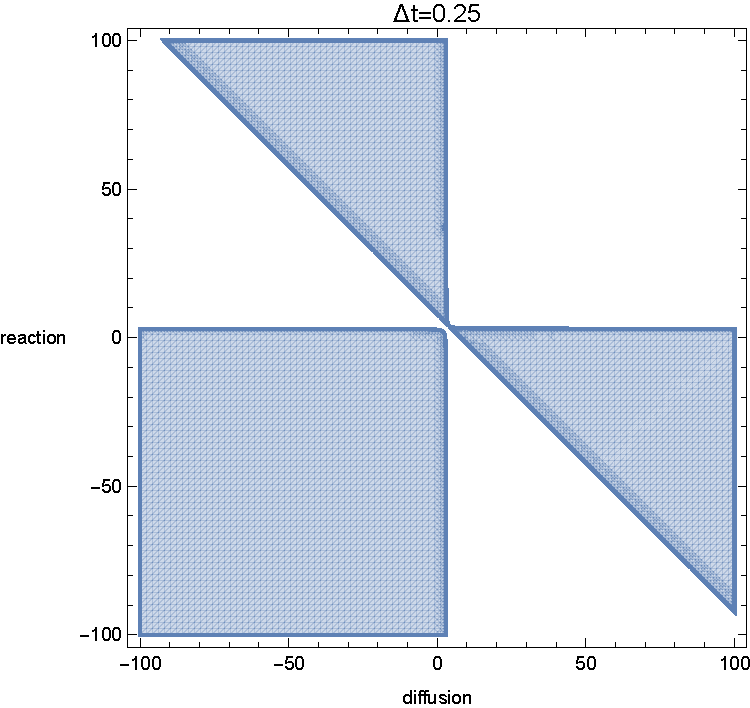
\includegraphics[width=0.4\textwidth]{misdc1} &   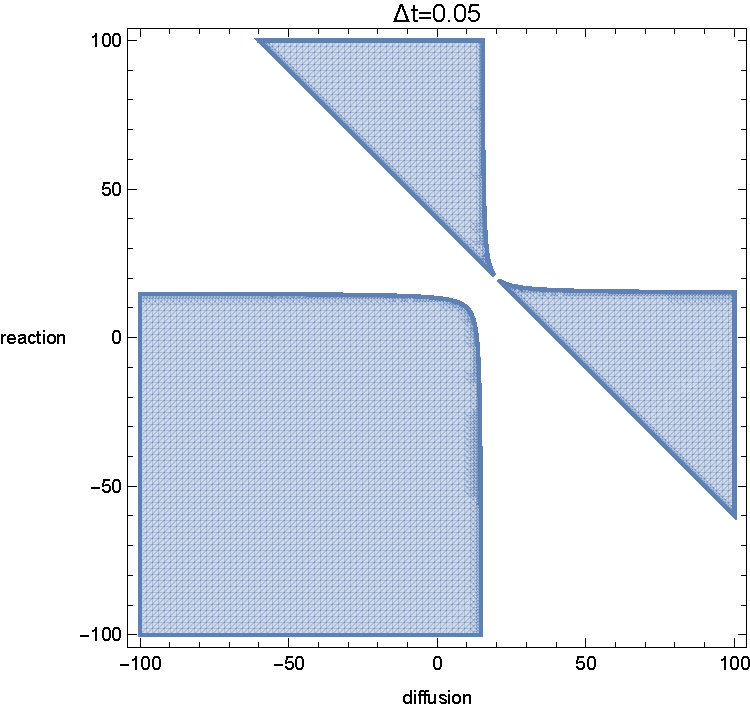
\includegraphics[width=0.4\textwidth]{misdc2} \\
(a) Classical MISDC, $\Delta t = 0.25$ & (b) Classical MISDC, $\Delta t = 0.05$ \\[6pt]
 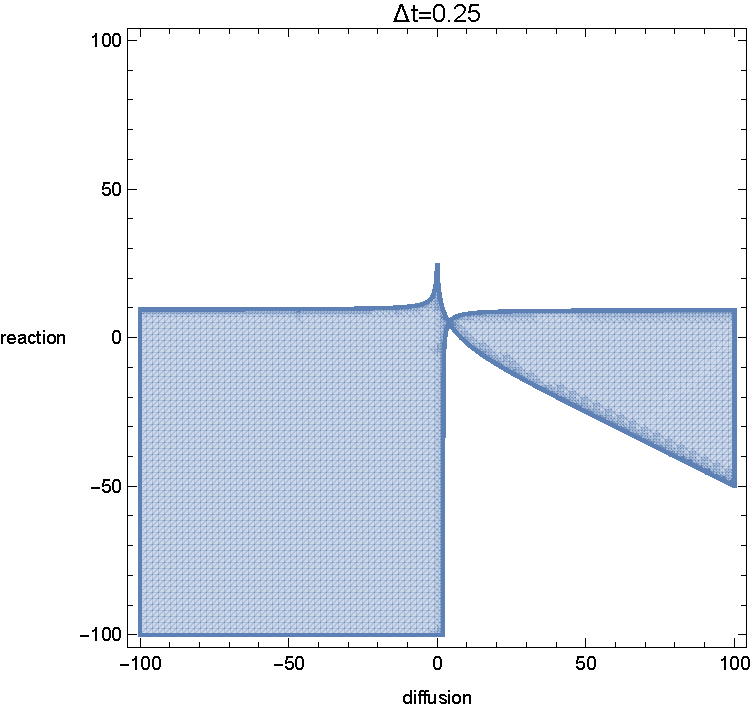
\includegraphics[width=0.4\textwidth]{const1} &   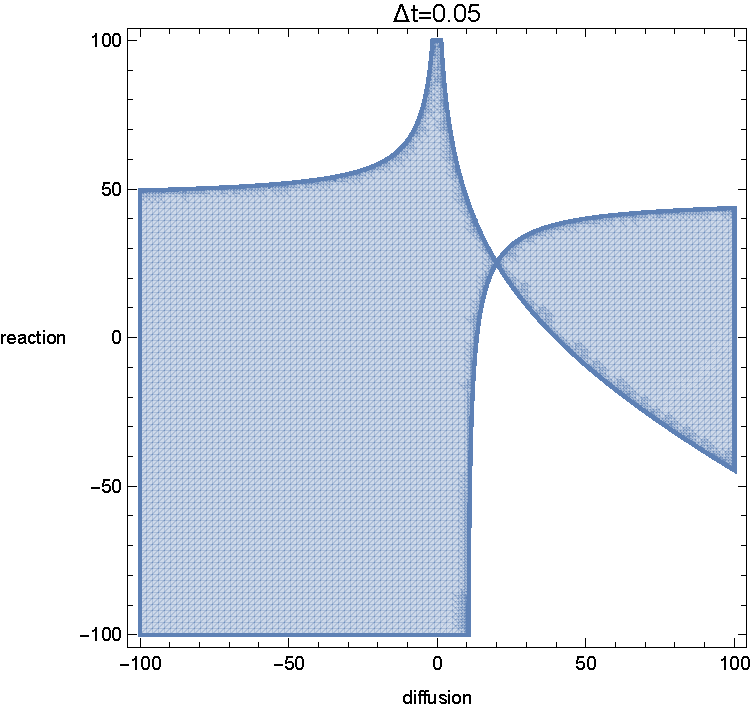
\includegraphics[width=0.4\textwidth]{const2} \\
(c) Constant forcing, $\Delta t = 0.25$ & (d) Constant forcing, $\Delta t = 0.05$\\[6pt]
\end{tabular}
\caption{Stability regions}
\end{figure}
\section{PDE}
To test a case more similar to the full LMC problem, we consider the PDE
\begin{equation}
    \label{pde}
    y_t = ay_x + \epsilon y_{xx} + ry(y-1)(y-1/2).
\end{equation}
Our spatial domain is the interval $[0, 20]$.
We enforce Dirichlet boundary conditions of $1$ on the left boundary, and 
$0$ on the right boundary, and use the initial condition
\[
    y(x, 0) = y^0(x) = \frac{\tanh(10-2x)+1}{2}
\]
We use the method of lines to solve this PDE, discretizing the first 
spatial derivative using the central difference operator, and discretizing 
the Laplacian using a three-point stencil. We are then left with an ODE of the 
form
\begin{equation}
    \label{mol-ode}
    y_t = A(y) + D(y) + R(y),
\end{equation}
where $A$ and $D$ are discretizations of the differential operators
\[
    a\frac{\partial}{\partial x},\qquad\epsilon \frac{\partial^2}{\partial x^2}
\]
respectively.

We then solve the ODE (\ref{mol-ode}) using an iterative MISDC scheme. I 
implemented the following variations:
\begin{enumerate}[i.]
    \item Classical MISDC using two advection nodes, quadrature based on 
        trapezoid rule;
    \item Classical MSIDC using four advection nodes, quadrature based on
        the interpolating cubic function;
    \item Solving the correction ODE using piecewise constant;
    \item Solving the correction ODE using piecewise linears;
    \item Solving the correction ODE using piecewise cubics.
\end{enumerate}
In this example, we can obverse very similar stability properties to those 
seen in the full LMC code. In particular, using a piecewise linear forcing term 
results in a ``less stable'' method than using a piecewise constant forcing 
term. Additionally, using a piecewise cubic forcing term appears to be so 
unstable as to be practically useless.

\subsection{Another ODE}
It also may be relevant to study an ODE of the form
\[
    y_t = ay + dy + r(y - 1/2),
\]
where both $d$ and $r$ are chosen to be negative. In this case, the balance 
between $d$ and $r$ will determine the equilibrium point to which the 
solution will decay.

I think that the stability analysis from section \ref{stability-analysis} when 
applied to this problem results in the same factors of $\alpha$. Since the 
stability regions all include the entire lower-left quadrant, all the MISDC 
methods appear to be stable for any choice of coefficients ($d,r < 0$). 
Numerical experiments agree with this result.

\section{Ideas for higher-order methods}
In order to increase the overall order of accuracy of the MISDC method, we need 
to increase the order of the quadrature rule used (and therefore, the number of 
substeps used for advection).

Our initial attempt to move to higher order was to change the forcing term in 
the correction ODE to a higher-degree polynomial corresponding to the 
interpolating polynomial used in the quadrature rule. Numerical experiments in 
the case of the linear ODE and the full LMC code indicate that this does not 
seem to be a very fruitful approach.

There are several other ideas for a potential higher-order method.
\begin{enumerate}[I.]
    \item  Use the ``classical MISDC'' Backward Euler step together with a 
           higher-order quadrature rule \label{high-order-misdc}
    \item  Use a constant forcing term when solving the correction ODE, where 
           the constant is given by the value of the quadrature over the 
           corresponding subinterval. \label{const-ode-quadrature}
\end{enumerate}
In both these cases, it is interesting to consider both Gauss-Lobatto and 
Gauss-Radau quadrature rules.

\subsection{Analysis of method \ref{high-order-misdc}}
As in section \ref{stability-analysis}, we can analyze the convergence 
properties of the iterative scheme. We consider the method with two time sub-%
steps.
\begin{align*}
    t_{(0)} &= t^n\\
    t_{(1)} &= t^n + \Delta t_1\\
    t_{(2)} &= t^n + \Delta t = t^{n+1},
\end{align*}
where the intermediate timestep $\Delta t_1$ is chosen to be the appropriate 
Gauss-Radau quadrature point. In our case we choose $\Delta t_1 = 2\Delta t/3$. 
For any function $z$, we use the notation
\begin{align*}
    z(t_{(1)}) &= z_1\\
    z(t_{(2)}) &= z_2.
\end{align*}
Our quadrature rule is then given by
\begin{align}
    I_{t_{(0)}}^{t_{(1)}}(z) &= \frac{9 z_1 - z_2}{16} \Delta t \label{qr-1}\\
    I_{t_{(1)}}^{t_{(2)}}(z) &= \frac{3 z_1 + 5 z_2}{16} \Delta t. \label{qr-2}
\end{align}
Notice that this quadrature rule is independent of the value of the function at 
time $t^n$. In other words, this is a Gauss-Radau quadrature rule, including 
only the right end-point as a quadrature point.

Using the standard MISDC algorithm to compute the solution at times $t_{(1)}$, 
and $t_{(2)}$, we can write
\[
    \left\| y^{(k+1)}_2 - y^{(k)}_2 \right\| = 
        \alpha \left\| y^{(k+1)}_1 - y^{(k)}_1 \right\|
      + \beta  \left\| y^{(k)}_2 - y^{(k-1)}_2 \right\|
\]
and
\[
\left\| y^{(k+1)}_1 - y^{(k)}_1 \right\| = 
        \gamma \left\| y^{(k)}_1 - y^{(k-1)}_1 \right\|
      + \delta \left\| y^{(k)}_2 - y^{(k-1)}_2 \right\|.
\]
Here, $\alpha, \beta, \gamma,$ and $\delta$ are algebraic expressions in terms 
of $a$, $d$, $r$, and $\Delta t$.
We can therefore see that a \textit{sufficient} (but not necessary) condition 
for the iterative scheme to converge is
\[
    |\alpha|, |\beta|, |\gamma|, |\delta| < 1.
\]
Setting $a = 0$ for simplicity, and plotting the region
\[
    \{ (d, r) \in \mathbb{R}^2 : |\alpha|, |\beta|, |\gamma|, |\delta| < 1. \}
\]
for some fixed $\Delta t$ gives us a region in which the iterative scheme 
is guaranteed to converge.
\begin{figure}[H]
\begin{tabular}{cc}
  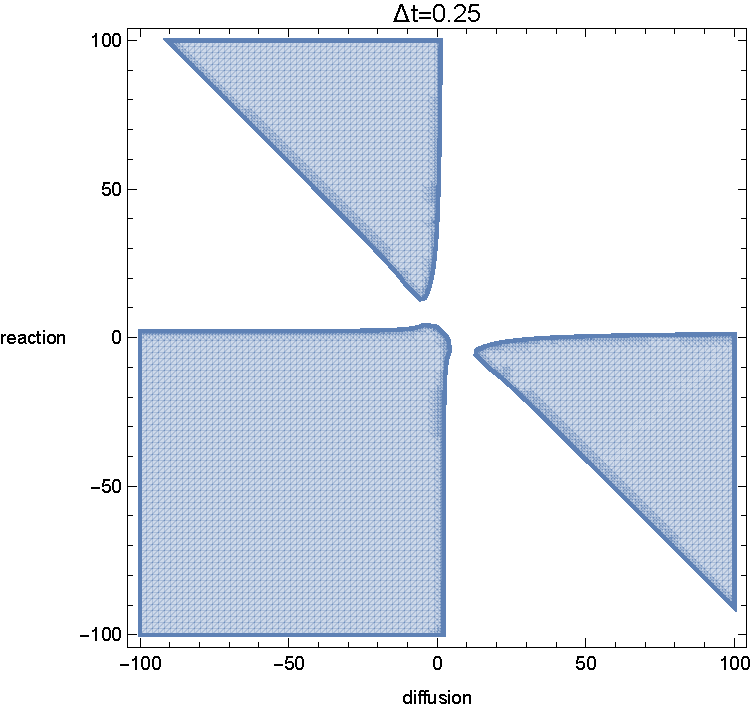
\includegraphics[width=0.4\textwidth]{radau1} &   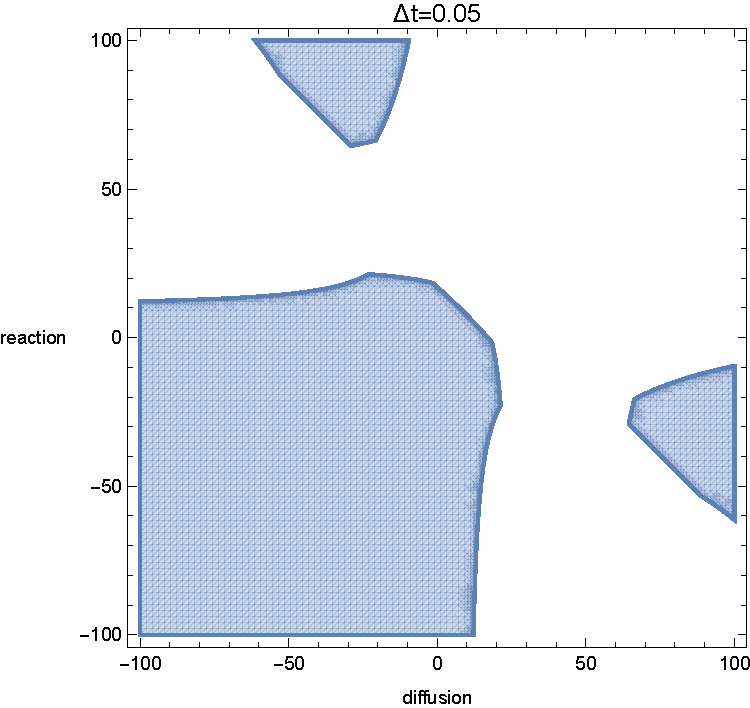
\includegraphics[width=0.4\textwidth]{radau2} \\
(a) $\Delta t = 0.25$ & (b) $\Delta t = 0.05$ \\[6pt]
\end{tabular}
\caption{Stability regions for MISDC with Radau quadrature}
\end{figure}
It is not clear if the choice of Radau quadrature rules over Guass-Lobatto has 
a significant effect on the stability regions of the method.
\subsection{Method \ref{const-ode-quadrature}}
Another potentially promising method is to solve the final correction equation 
with an ODE solver, but instead of represting the forcing term as the 
interpolating polynomial, we choose to represent the forcing term as a piecewise 
constant, whose value is given according to the quadrature rules (\ref{qr-1}) 
and (\ref{qr-2}).

It still remains to perform the stability analysis for this scheme, and it is 
not certain that this will provide the desired increase in order of accuracy.

Implementing this method for the case of the ODE from section \ref{sec:ode}, 
I was not able to attain higher-order of accuracy using this method. 
I susepct that in order to increase the order of accuracy, the degree of 
polynomial used in the forcing term would need to be increased.

\subsection{Radau vs. Lobatto quadrature in method \ref{high-order-misdc}}
Analysing the stability regions for method \ref{high-order-misdc}, it does 
not appear that there are significant differences when choosing to use either 
Gauss-Radau or Gauss-Lobatto quadrature rules. For this reason, it appears 
to be advantageous to choose to use Gauss-Lobatto quadrature: the left endpoint 
of the interval of integration is always known, so it is possible to perform a 
three-point quadrature by calculating the solution at only one intermediate 
point. On the other hand, if we were to use a Gauss-Radau rule, and to not 
include the left endpoint as one of our quadrature points, we would have to 
calculate the solution at \textit{two} intermediate points in order to perform 
a three-point quadrature.

In the case of a Gauss-Lobatto quadrature, the values of 
$\alpha, \beta, \gamma,$ and $\delta$ such that
\begin{align}
    \left\| y^{(k+1)}_2 - y^{(k)}_2 \right\| &= 
        \alpha \left\| y^{(k+1)}_1 - y^{(k)}_1 \right\|
      + \beta  \left\| y^{(k)}_2 - y^{(k-1)}_2 \right\|\\
    \left\| y^{(k+1)}_1 - y^{(k)}_1 \right\| &= 
        \gamma \left\| y^{(k)}_1 - y^{(k-1)}_1 \right\|
      + \delta \left\| y^{(k)}_2 - y^{(k-1)}_2 \right\|
\end{align}
are given by:
\begin{align*}
    \alpha &= \Delta t
        \frac{3(-45(d+r) + (7d^2 -22dr + 7r^2)\Delta t 
            + 11dr(d+r)\Delta t^2)}
        {4d\Delta t - 3)(2d\Delta t - 3)(r\Delta t - 3)(2r\Delta t - 3)}\\
    \beta &= \Delta t
        \frac{2(r(7r\Delta t - 27) + d(r\Delta t(-7r\Delta t + 27) - 27) 
            + d^2\Delta t(r\Delta t(2r\Delta t - 7) + 7)) }
        {d\Delta t - 3)(2d\Delta t - 3)(r\Delta t - 3)(2r\Delta t - 3)}\\
    \gamma &= \Delta t\frac{2(d+r)+dr\Delta t}{(d\Delta t - 3)(r\Delta t - 3)}\\
    \delta &= \Delta t\frac{4(d+r)}{3(d\Delta t - 3)(r\Delta t - 3)}.
\end{align*}
\end{document}
